%!TEX root = mainfile.tex

\subsection{Euclid} % (fold)
\label{sub:euclid}

	\subsubsection{Mission Overview} % (fold)
	\label{ssub:mission_overview}
		The Euclid mission is planned for launch in 2018\cite[p.~8]{Euclid_Definition_Study_Report} at an estimated total cost of 800\,million Euros, and will work in the optical and near infrared\cite{bbc_euclid}. Its primary goal is to conduct a wide survey, some 15000\,degrees of sky is planned to be covered, in order to map the geometry of the dark universe. It will look at galaxies and galaxy clusters to work out their redshifts and shapes, back to $z=2$. There is also to be a deep survey which is expected to cover around 40\, degrees of sky to a depth 2 magnitudes deeper than the wide survey. This deep survey will allow astronomers to see even further back in time, up to redshifts of 8 and potentially even higher. The primary mission objectives are expected to be completed within 7 years.

		One of Euclid's main scientific objectives with the deep survey is to study high redshift galaxies at $z\ge6$ over a very wide survey area. This will give astronomers the opportunity to spectroscopically confirm hundreds of galaxies for use in the study of the EoR. It will help constrain the bright end of the luminosity function at high z. Euclid will ``detect hundreds of $z=7$ galaxies brighter than an apparent magnitude $J=26$ and tens at $z$ greater than 8''\cite{Euclid_Definition_Study_Report}.

		Another is to study clusters of galaxies in the near IR as well as the visible; a weak gravitational lensing survey (as discussed in section~\ref{sec:gravitational_lensing}) will be carried out, looking for disturbances and distortions in the light from galaxies as a result of large amounts of mass perturbing the path of the photons emitted from them. ``Euclid measures the shapes of 30 resolved galaxies per arcmin$^2$ in one broad visible R+I+Z band (550--920\,\si{\nano\metre}) down to AB mag 24.5''\cite[p.~9]{Euclid_Definition_Study_Report}.
	% subsubsection mission_overview (end)

	\subsubsection{Capabilities} % (fold)
	\label{ssub:euclid_capabilities}
		\begin{itemize}
			\item Visual Imaging/ Photometry, 550--900\si{\nano\metre}
			\item Spectroscopy, 1100--2000\si{\nano\metre}
			\item NIR Imaging/ Photometry, 920--2000\si{\nano\metre} (Y, J,H bands)
		\end{itemize}

		Euclid will have two instruments in order to do the above; a wide-band imaging system in the visible (VIS), and an instrument capable of both slit-less spectroscopy as well as NIR imaging (NISP). These instruments will be able to operate simultaneously when required.
	% subsubsection capabilities (end)

	\subsubsection{Method of Conducting Deep Survey} % (fold)
	\label{ssub:method_of_conducting_deep_survey}
		The Euclid deep survey will be carried out by re-visiting particular areas in the wide survey over an extended period of time. Over this time, the depth will be built up by combining a series of images taken of the same piece of sky (known as stacking). The wide survey will reach the required magnitude depth with one exposure, but to reach 2 magnitudes deeper (26th magnitude AB at 5 sigma) considerably more exposures will be needed. Figure~\ref{fig:euclid_visits_magnitude} shows the number of visits to increase the depth to 26th magnitude. The current estimate is that this will take around 36 exposures, and it has been decided to do 40 to make sure\cite{NISP_Performance_Analysis_ReportEUCL}. The telescope operates a 4 step dithering mode so that if there are faulty pixels or systematic errors, the image is still usable.
		\begin{figure}[!htb]
			\begin{center}
				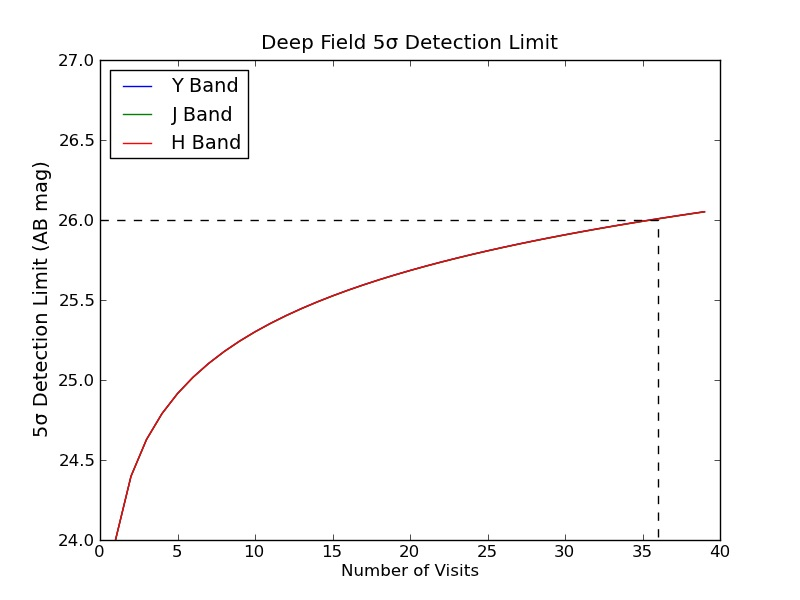
\includegraphics[width=0.62\textwidth]{../Images/Euclid_visits_magnitude.jpg}
			\end{center}
			\caption{Number of visits required to meet the Euclid's goal of a depth of 26th magnitude.\label{fig:euclid_visits_magnitude}}
		\end{figure}
	% subsubsection method_of_conducting_deep_survey (end)

	\subsubsection{Uses and Limitations For Euclid's Use In Studying High Redshift Galaxies} % (fold)
	\label{ssub:uses_and_limitations_for_euclid_s_use_in_studying_high_redshift_galaxies}
		The main limitation of using Euclid for this study is its filter range: Since the drop out technique requires two filters above the drop and one below, the redshift of the galaxy must be such that the filters available are able to achieve this. Euclid's longest wavelength filter is centred at \SI{1.63}{\micro\metre} (J-band filter). If the drop is at too long a wavelength, only one band will observe flux. Without two bands observing flux, no colour-colour diagrams can be plotted, and one measurement of flux and another of no flux is not enough to have confidence that the object is a Lyman break galaxy. Table~\ref{fig:euclid_ir_filters} shows the IR filters of Euclid, along with each filter's central wavelength and it's bandwidth.
		\begin{table}[ht]
			\centering
				\begin{tabular}{c|c|c}
					Filter & Central Wavelength & Bandwidth \\
					\hline\hline
					Y (920--1146) & 1020 & 226 \\
					H (1146--1372) & 1220 & 226 \\
					J (1372--2000) & 1630 & 628 \\
				\end{tabular}
				\caption{Euclid space telescope IR filters.\label{fig:euclid_ir_filters}}
		\end{table}

		From this, it can be concluded that the survey will be unhelpful in determining galaxies past a redshift of 10.5 (corresponding to the drop being observed at \SI{1.40}{\micro\metre}): The object would be detected in the J band, but not in either H or Y. The end of the H filter and start of the J filter is at \SI{1.37}{\micro\metre}. To get significant flux in the Y band, ideally the galaxy would need to be at a redshift of 10 or lower, such that a noticeable amount of flux was detected in H.

		A weak lensing survey is planned with Euclid. This will help find gravitational lenses which could be used to magnify very faint Lyman break galaxies at high redshift. From this weak lensing survey, the strongest lenses could be selected and used as targets for other telescopes such as JWST or ELT to study more closely to see if any high redshift LBGs lay behind.

		The spectroscopic mode can be used (grism spectroscopy) to determine the redshift of LBGs as outlined in section~\ref{sec:lyman_break_galaxies}. The advantage of grism spectroscopy is that multiple objects can be studied simultaneously, meaning if there are multiple likely candidates in the field of view, their spectra can all be gathered at once, reducing the overall time taken to study a large number of redshift galaxies. This is particularly useful to Euclid, which has a wide field of view of just over 0.5 square degrees, increasing the chance of multiple candidates.
	% subsubsection uses_and_limitations_for_euclid_s_use_in_studying_high_redshift_galaxies (end)

	\subsubsection{Key Technical Data} % (fold)
	\label{ssub:key_technical_data}
		The data in table~\ref{tab:Euclid_technical} is quoted for the deep survey NIR photometry. Some data is subject to slight change as the planning stages progress.
		\begin{table}[ht]
			\begin{center}
				\begin{tabular}{l|l}
					Component & Details \\
					\hline\hline
					Primary mirror		& \SI{1.2}{\metre} \\ \hline
					FoV 				& $0.763\times0.763$\,deg$^2$ \\ \hline
					Pixel size			& \SI{0.3}{\arcsecond}$\times$\SI{0.3}{\arcsecond} \\ \hline
					Detector Array		& \num{2000}$\times$\num{2000}\,\si{\pixel} \\ \hline
					Resolution 			& 0.3 to \SI{0.6}{\arcsecond} (in J band) \\ \hline
					Plate Scale (infrared)	& \SI{0.3}{\arcsecond\per\pixel}
				\end{tabular}
			\end{center}
			\caption{Technical data for the deep survey NIR photometry\cite{Euclid_Definition_Study_Report}.\label{tab:Euclid_technical}}
		\end{table}
	% subsubsection key_technical_data (end)
% subsection euclid (end)
